\documentclass{article}
\usepackage[UTF8]{ctex}
\usepackage{geometry}
\usepackage{multirow}
\usepackage{natbib}
\geometry{left=3.18cm,right=3.18cm,top=2.54cm,bottom=2.54cm}
\usepackage{graphicx}
\pagestyle{plain}	
\usepackage{setspace}
\usepackage{enumerate}
\usepackage{caption2}
\usepackage{datetime} %日期
\renewcommand{\today}{\number\year 年 \number\month 月 \number\day 日}
\renewcommand{\captionlabelfont}{\small}
\renewcommand{\captionfont}{\small}
\begin{document}

\begin{figure}
    \centering
    
\includegraphics[width=8cm]{upc.png}

    \label{figupc}
\end{figure}

	\begin{center}
		\quad \\
		\quad \\
		\heiti \fontsize{45}{17} \quad \quad \quad 
		\vskip 1.5cm
		\heiti \zihao{2} 《计算科学导论》个人职业规划
	\end{center}
	\vskip 2.0cm
		
	\begin{quotation}
% 	\begin{center}
		\doublespacing
		
        \zihao{4}\par\setlength\parindent{7em}
		\quad 

		学生姓名:\underline{\qquad  张一帆 \qquad \qquad}

		学\hspace{0.61cm} 号:\underline{\qquad 1907010214\qquad}
		
		专业班级:\underline{\qquad 本研人工智能 \qquad  }
		
        学\hspace{0.61cm} 院:\underline{计算机科学与技术学院}
% 	\end{center}
		\vskip 1.5cm
		\centering
		\begin{table}[h]
            \centering 
            \zihao{4}
            \begin{tabular}{|c|c|c|c|c|c|c|c|c|}
            % 这里的rl 与表格对应可以看到,姓名是r,右对齐的;学号是l,左对齐的;若想居中,使用c关键字。
                \hline
                \multicolumn{5}{|c|}{分项评价} &\multicolumn{2}{c|}{整体评价}  & 总    分 & 评 阅 教 师\\
                \hline
                自我 & 环境 & 职业 & 实施 & 评估与 & 完整性 & 可行性 &\multirow{2}*{} &\multirow{2}*{}\\
                分析& 分析& 定位 & 方案 & 调整 & 20\% & 20\% & ~&~ \\\            
                10\% & 10\% & 15\% & 15\% & 10\% & &  &~ &~\\
                \cline{1-7} 
                & & & & & & & ~&~ \\
                & & & & & & & ~&~ \\
                \hline      
            \end{tabular}
        \end{table}
		\vskip 2cm
		\today
	\end{quotation}

\thispagestyle{empty}
\newpage
\setcounter{page}{1}
% 在这之前是封面,在这之后是正文
\section{自我分析}
	人的一生有两个极其重要的分水岭,可以说是成功与否的转折点。第一个是幼儿启蒙时期,这个时候是培养一个人优良人格的最好时机;第二个则是青年时期,而我们大学生正处于这样一个特殊的时期。大学生如正午烈阳一般,智力、体力都处于最顶峰的时期,这个时间段学习能力也是最强的,所以我们更不能荒废了这无比宝贵的几年。可我们也是很迷茫的,刚从高考战场中“脱身”出来,陡然接收了大学铺天盖地的社团、课程等信息,让我们措手不及。而如何选择自己的学习方向,合理安排以后的学习生活时间呢?这样一份个人规划便必不可少了。\par
\subsection{自然条件}
我叫张一帆,今年19岁,我来自湖南长沙,现在在青岛读大学,是一个阳光活泼的男生,平时热爱搞运动,所以有一副强劲的体魄。\par
\subsection{性格分析}
也许是因为家庭环境的影响 ,我性格比较随和,能很快地融入新环境中。在以前的时候我非常自卑,很内向,而后来可能是因为喜欢搞运动吧,我发现我很喜欢和别人交流,慢慢地,我就变得外向起来,善于与人交流。作为刚踏入大学的“fresh man”,我对一切事物都非常感兴趣,也乐于参与。我不喜欢一成不变的重复循环,我喜欢挑战自我,注重实用性,愿意接受新事物并对其进行归纳总结。所以我当初报考了计算机专业,我觉得这个专业非常适合我。\par
\subsection{教育与学习经历}
我小学就读于长沙市重点小学砂子塘小学,毕业后就读于稻田中学,成绩优异,并通过中考6A,考入国家重点中学长沙市四大名校之首的雅礼中学,最后来到211高校中国石油大学华东校区继续学习,学习的是计算机科学与技术专业,并选入人工智能本研一体班。\par
\subsection{工作与社会阅历}
我小学时曾当过长沙晚报小记者,出过很多活动,有采访与写稿方面的经验。在高中时我曾出任16届长沙市雅礼中学羽毛球社的社长,举行过大小会议若干。在2017年暑假我与长沙市几所中学的羽毛球社长共同创办了长沙市羽毛球中学社团联盟,并担任副主席职位。在我在任的两年里,共举办了四次联赛,并带领雅礼羽协蝉联四届冠军。\par
\subsection{知识、技能与经验}
我热爱学习,刻苦努力,从小学到高中,学习成绩优异,深受老师同学们的欣赏。我已熟练掌握中学理科的知识与思想,并能加以适当拓展运用。我最擅长的技能是:推理能力、组织能力、团队协作能力。英语方面,我也参加过许多赛事,词汇量处于高考水平与四级之间,能用英语进行日常的交流,以及能够阅读外文文献。为响应国际号召,我从小就立志成为一个创新型人才,参加了各种创新大赛,具有一定的创新能力。\par
\subsection{兴趣爱好与特长}
我阳光开朗,善于交朋友。我从小就爱好运动,喜欢篮球、乒乓球、排球等球类运动,尤其擅长羽毛球。从小我就开始在兴趣班接受羽毛球训练,目前在校队训练,也算是小有所成了吧。音乐方面,我喜欢吉他和单簧管。学习方面,我对编程也情有独钟,敢于探索新的知识,善于从网络上汲取新知识。\par
\section{环境分析}

\subsection{社会环境分析}
当今社会,在经济全球化的引领下,第三次科技革命正在如火如荼地进行中,科技已成为评判国家综合国力的一大重要标准。世界上各大名企公司,也无不乘着科技这艘巨轮破浪而行。华为公司为何能取得成功,就是因为在它18万员工中,百分之四十五的都是科研人员,每年的研发投入占营销总额百分之十五。而人工智能则是现在的一大热门浪潮。世界各国投入大量资金大力发展与人工智能相关的高科技前沿技术,人工智能方面的高水平人才正处于急缺的现状。所以,每年毕业的计算机专业学生特别是人工智能专业的学生人数虽然很多,但基本也处于供不应求的状况,水平突出的学生各大公司企业更是抢着要。我们正处于这样一个大变革时代!\par
\subsection{家庭环境分析}
我出生部分于一个医学世家,我的大亲戚都从事与医学相关的工作。我们家经济收入水平中等,属于普通工薪家庭。我家人一开始是想要我学医的,不过我还是遵循了我自己的选择,报考了计算机专业。如果以后从事如智慧医疗方面的工作的话,我有足够的优势。\par
\subsection{职业环境分析}
据我国权威部门预测表明,随着我国经济与社会的发展,科学技术的进步,今后几年对专门人才的需求将有较大的变化。当代任何一个国家,要在高科技领域占据主导地位,必须拥有相当规模的杰出科学家,并使科学家队伍平均年龄尽量接近“最佳年龄区”。 据权威调查统计,重大科学发现的最佳年龄峰值为37岁,最佳年龄区为<25~45岁。可见高科技人才竞争的焦点是年轻科学家。目前我国已实施“长江学者奖励计划”,其目的就是使中青年拔尖人才脱颖而出。这其中就包括计算机与人工智能方面的人才。目前各大IT公司的工作环境都趋于优越,但对于人才的水平要求也越来越高,尤其是创新能力。总的来说,人工智能的职业前景非常好。\par
\newpage
\begin{figure}[h!]
	\centering
	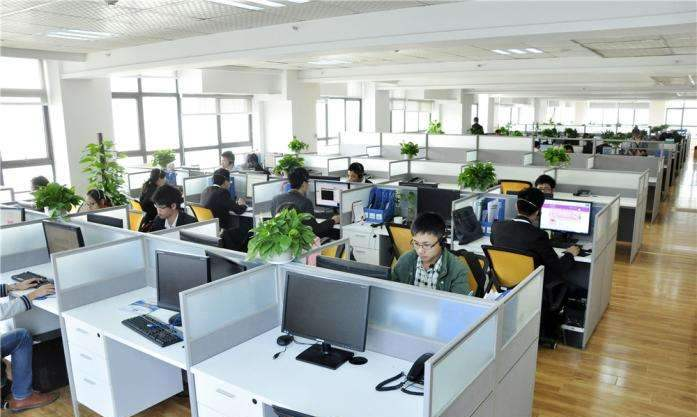
\includegraphics[scale=0.7]{it.png}
	\caption{IT行业工作环境}
	\label{fig:sss}
\end{figure}


\subsection{地域与人际环境分析}
对于我目前来说,未来可供选择的城市有两个,一个就是留在青岛深造,一个是回长沙工作。对于青岛来说,气候非常好,沿海,IT企业众多,是高科技行业的沃土。而回长沙的优势是人脉资源丰富,不过长沙深处内陆,对于高新技术的接触机会较少。\par
\par 




\section{职业定位}


\subsection{行业领域定位与理由}
基于我就读与人工智能本研一体班的现状,我在未来大概率会从事人工智能方面的工作。又因为我出生于医学世家,所以我想尝试往智慧医疗这方面发展。智慧医疗也是一个比较热门的方向,我家人工作的医院也有发展智慧医疗的项目,如果我未来真的从事这方面研究,在就业方面会比他人更有优势,这是目前我考虑的重要因素。\par
\subsection{职业岗位起点定位与理由}
俗话说得好,“不想当将军的士兵不是好士兵“,但对于我的职业岗位起点,我并不会好高骛远、眼高手低,我觉得不用一开始就想着直接能进入公司高层。而且许多学计算机的同学都想毕业后立马就进入高薪外企,但是首先,这个几率比较小,再者,作为刚刚毕业的小白,我们不一定能适应外企那种高强度的工作氛围。我觉得适合自己才是最好的,我接受从普通员工以上的岗位作为我的职业起点。\par
\subsection{职业目标与可行性分析}
\par

\begin{enumerate}[(1)]
	\item 短期目标
	
	\begin{table}[!htbp]   
		 \newcommand{\tabincell}[2]{\begin{tabular}{@{}#1@{}}#2\end{tabular}}
		 \centering
		\begin{center}  
				\renewcommand{\arraystretch}{2}
			\begin{tabular}{|c|c|c|c|}  
				\hline  
				年级 & 致力方向 & 目的 & 具体目标 \\ \hline  
				大一& \tabincell{c}{C语言、数分、\\线代等基础课程} & \tabincell{c}{打好坚实的基础,\\培养学习兴趣与数学思维}& \tabincell{c}{拿到全国大学生英语四级证书;\\各门课程综测达到七十以上 } \\ \hline  
				大二 & \tabincell{c}{基础课程、专业课 \\ 程和活动相结合为\\主,兼职实践为辅} & 为大三学习专业知识提供基础 & 拿到全国大学生英语六级证书 \\  
				\hline  
				大三 & 专业知识学习 & 提高专业知识水平 & \tabincell{c}{参加各项专业竞赛;关注与计算机专业\\ 和人工智能相关的研究生方向} \\ \hline
				大四 & \tabincell{c}{跟随导师做项目;\\实习} & 了解IT企业的
				运作 & 初步确定自己心仪的公司 \\ 
				\hline
			\end{tabular}  
		\end{center}  
	\end{table}
	\item 中长期目标
	\begin{itemize}
		\item[i)]本科毕业之后继续在中国石油大学读人工智能专业研究生,并积极跟随导师进行与智慧医疗方面相关的课题研究。
		\item[ii)]研究生毕业后进入一所知名大企业工作,成为一名正式员工。
		\item[iii)] 努力工作,建立良好的交际网,努力在领导面前表现自己的才能,博取提升的机会。
		\item[iiii)] 确立自己的人生观、价值观和人生目标。人生规划的目的就是要实现自己的人生目标,也是人生规划的基础和原则。人的人生观、价值观和人生目标会随年龄的增长、对社会的认识不断的改变和清晰。人生规划也应该随之进行相应的调整与改变。
	\end{itemize}
\end{enumerate}




\section{实施方案}
在明确了职业定位后,要制定实现职业生涯目标的行动方案,不付诸行动,职业目标只能是一种梦想。实施方案是实现职业目标的保证,尽量考虑周全、具有可操作性。\par
而我的实施方案分为以下几个方面:\par
\begin{enumerate}[1、]
	\item 目前我的优势科目为英语,我应该再接再厉提高英语水平,争取难得的出国交流机会;我的创新思维与数学思想不错,以后积极参加一下创新科技方面的竞赛,积累经验。
	\item 我的缺点是定力不足,比较懒散。我以后应该制定好每日任务,对待任务要积极思考,严格要求自己。
	\item 友善待人,处理好自己的人际关系,为实现职业生涯目标打下基础。
	\item 合理分配时间,平衡工作学习与家庭生活的关系,做到两不误。
	\item 平时多锻炼身体,调整心态。如果感觉到工作压力大,就约朋友一起出去打打球,放松心情,储备力量,为之后的努力而准备。
\end{enumerate}
\par 

\section{评估与调整}

\subsection{评估时间}
初期每个学期评估一次,时间长了之后可以延长评估时间间隔,大概每学年评估一次\par
\subsection{评估内容}
做好记录,当学年定下的任务与具体目标是否按量按质完成,对于已完成的目标记录心得体会与收获,对于未完成的目标,及时规划时间,尽快将其完成。提前准备下一学年的目标。\par
\subsection{调整原则}
社会是不断变化的,事情也不会一成不变,但我一定会朝着我的目标坚定前行。所以,适当的调整是不可避免的。如果当学年本应完成的目标但未达成,经过评估发觉其已不适应我的现状,可以适当将其缩减或删去;根据实际情况,调整未来的学习工作目标。\par




\end{document}
